\appendix

\chapter{Preprocessing}
\subsubsection{Normalization}
This step is done to avoid the variations in amplitude between sound recordings from different devices.
\begin{equation*} x_i = x_i - x_{mean} \end{equation*}

\subsubsection{Trimming}
This step is necessary to save computational resources from being spent on unvoiced parts of the signal. Hence, silent parts of the signal should be removed. The trimming is done using the algorithm in \cite{Saha_anew}. This algorithm uses the background noise features to set thresholds, hence no need to assume any ad-hoc values. If $d$ (Mahalanobis distance) of a sample comes out to be lesser than 3, it is rejected. $b_{mean}, b_{sd}$ are the Gaussian parameters of the background noise.
\begin{equation*} d = x - b_{mean} / b_{sd} \end{equation*}

\subsubsection{Pre-emphasis}
Due to the nature of the glottal impulse, the human speech has more energy in the lower frequencies. Hence, the signal is applied with pre emphasis filter (a first order high pass filter) that boosts the higher frequencies.
\begin{equation*} x_i = x_i - \alpha x_{i-1} \end{equation*}

This enables the acoustic models to gain more information from the higher formants. $\alpha = 0.95$ has been taken for our system. 

\subsubsection{Framing and Hamming Window}
We want to extract features from a small window of speech that represents a sub phoneme. To convert the signal to a stationary signal frame wise, a hamming window is applied on each frame. It disallows discontinuity by suppressing the boundaries of the signal. One of the most commonly used hamming window is:

\begin{equation*} w(i) = 0.54 - 0.46\frac{2\pi(i - 1)}{N - 1}, \quad \begin{aligned} 1 \leq i \leq N \end{aligned}
\end{equation*}

\chapter{Feature Extraction}
\section{LPCC}

Linear Predictive Coding is a very useful technique for encoding high quality speech at a low bit rates. It provides very accurate estimates of the speech parameters. Its main advantage comes from the fact that it is based on a simplified vocal tract model. LPC includes a speech production function mimicking the air from our lungs, and the error filter mimicking our larynx.

We find out the linear predictive cepstral coefficients (LPCC) using the autocorrelation method from \cite{rabinerbook}.

\subsubsection{Autocorrelation}
The first step is to find $p$ autocorrelation values for each frame of windowed signal using 

\begin{equation*} \sum_{n=0}^{n-1-m}{\tilde{x}_l(n)}{\tilde{x}_l(n+m)}, \quad \begin{aligned} m=0,1,...,p. \end{aligned} \end{equation*} 

$p$ is the linear prediction order.

\subsubsection{Durbin solve}
A $pXp$ Toeplitz matrix is created by using the above $p$ autocorrelation values. The Toeplitz matrix is solved using Durbin method to give the LPC coefficients:

\begin{equation*} E^{(0)} = R(0) \end{equation*}
\begin{equation*} k_i = \dfrac{R(i) - \sum_{j=1}^{i-1}\alpha_j^{i-1}R(|i-j|)}{E^{i-1}},  \quad \begin{aligned} 1 \leq i \leq p. \end{aligned} \end{equation*}
\begin{equation*} \alpha_i^{(i)} = k_i \end{equation*}
\begin{equation*}\alpha_j^{(i)} = \alpha_i^{(i-1)} - k_i\alpha_{i-1}^{(i-1)},   \quad \begin{aligned} 1 \leq j \leq i-1. \end{aligned}\end{equation*}
\begin{equation*} E^{i} = (1-k_i^2)E^{i-1} \end{equation*}

\begin{figure}[h!]
    \centering
    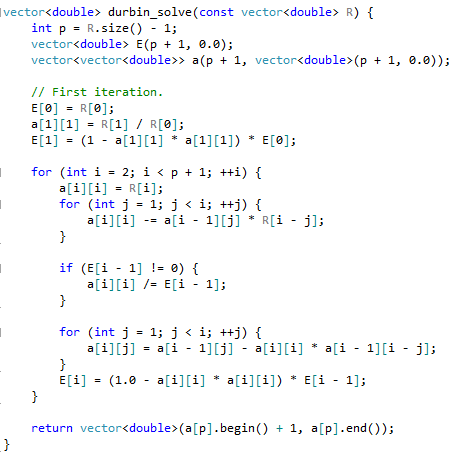
\includegraphics[scale=0.9]{sr-lib-durbin-code}
    \label{fig:sr-lib-durbin-code}
    \caption{Implementation of Durbin's solve}
\end{figure}

\subsubsection{Cepstral Coefficients}
In the last step, the LPC cepstral coefficients are derived from the LPC coefficients. $\sigma^2$ is the gain term of the LPC model.

\begin{equation*}
    c_0 = ln\sigma^2
\end{equation*}
\begin{equation*}
    c_m = a_m + \sum_{k = 1}^{m - 1}(\frac{k}{m})c_ka_{m-k}, 
    \quad \begin{aligned} 1 \leq m \leq p. \end{aligned}
\end{equation*}
\begin{equation*}
    c_m = \sum_{k = 1}^{m - 1}(\frac{k}{m})c_ka_{m-k}, 
    \quad \begin{aligned} m > p. \end{aligned}
\end{equation*}

LPCC are proved to be more robust than LPC. A sine window is applied over these cepstral coefficients to desensitize them towards noise and noise like sounds.

\section{MFCC}

MFCC is one of the most popular feature extraction technique. MFCC aims to mimic the human hearing by penalizing higher frequencies and boosting lower frequencies. The mapping between Hertz and Mel is logarithmic above 1000Hz and linear below 1000 Hz. The Mel scale is based on an empirical study conducted by Stevens and Volkmann.

\begin{equation*} m = 2595 log_10 (1 + \frac{f}{700}) \end{equation*}

\subsubsection{DFT}
The frequency spectrum is extracted by finding the Discrete Fourier Transform (using FFT) of each frame. We implement the FFT using Cooley-Tukey, in-place, breadth-first, decimation-in-frequency algorithm described in \cite{Blahut:1985:FAD:537283}.

\begin{figure}[h!]
    \centering
    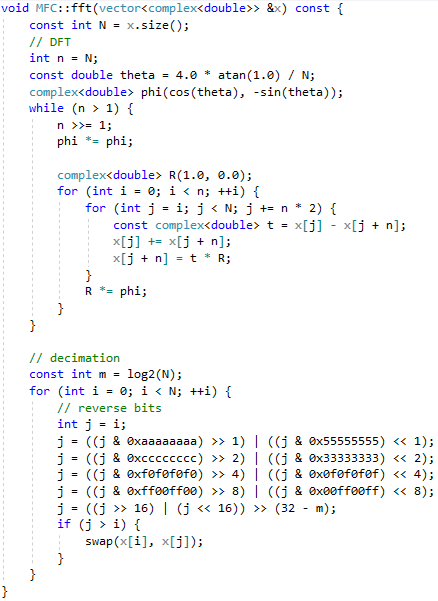
\includegraphics[scale=0.9]{sr-lib-fft-code}
    \label{fig:sr-lib-fft-code}
    \caption{Implementation of FFT}
\end{figure}

\subsubsection{LMFB}
This step is performed by using filter banks with filters centered according to the Mel frequencies.  We have used 40 filter banks in our implementation.

\subsubsection{DCT}

Inverse Fourier Transform is done using Discrete Cosine Transform in this step. The result of this step are the Mel frequency cepstral coefficients.

\begin{equation*}
    c[m] = \sum_{i=1}^M logY(i)cos[\frac{m\pi}{M}(i - 0.5)]
\end{equation*}

$M$ is the number of filters, $c[m]$ are the cepstral coefficients, $Y(i)$ are the filter outputs.

\subsubsection{Normalization}

To reduce the channel effect of the recordings, cepstral mean subtraction is done. When people record from different channels, different channel effect is created. $Q$ is the number of cepstral coefficients.

\begin{equation*}
    c_i = c_i - c_{mean},
    \quad \begin{aligned} 1 \leq i \leq Q. \end{aligned}
\end{equation*}

\section{Derivative coefficients}

Co-articulation and irregularities in speech cause the speech signal to not be stationary frame to frame. To acknowledge this delta and delta delta (acceleration) features can be calculated from the cepstral coefficients.
We use the linear regression method to calculate the derivative features.

\begin{equation*}
    \Delta c_j[i] = \frac{\sum_{m=-M}^{M} m c_{j+m}[i]}{\sum_{m=-M}^{M} m_2 }
\end{equation*}

Now the complete feature set is:
{\begin{itemize}
\item Q cepstral coefficients (using LPCC or MFCC)
\item Q delta cepstral coefficients
\item Q acceleration cepstral coefficients    
\end{itemize}}

\chapter{Vector Quantization}

Vector Quantization was originally being used for data compression, but it performs well even for speech recognition. A large set of vectors are divided into groups such that they have almost equal number of neighbors closest to them. VQ vastly decreases the data that has to be processed. Instead of having full utterances and words as training data, we will be able to have only a small sized codebook.

\section{KMeans}
KMeans is one of the most basic and yet useful algorithm or clustering of data. The algorithm is described as:

\begin{enumerate}
\item Choose N random points as centroids
\item Assign all other points to one of the N centroids based on distance
\item Recalculate the centroids by using the above created buckets
\item Repeat from step 2 till the centroids converge
\end{enumerate}

\section{LBG}
Linde Buzo Gray algorithm solves one of the very important shortcomings of KMeans. It solves the initialisation problem. KMeans chooses N random points and can reach local optimal states. To overcome this LBG algorithm completely removing initial randomness by using the following steps:

\begin{enumerate}
    \item Start with number of centroids as 1 (the mean of all vectors)
    \item Split the centroids into two
    \item Optimize the centroids using KMeans
    \item Repeat from step 2 till the desired size of centroids is reached
\end{enumerate}

\chapter{Word Modeling}

Now the feature extraction is done on input signals and then using the codebook, the closest bucket is found for each frame. This greatly reduces the amount of data that we have to process. These bucket values are referred to as the observations. HMM has a number of hidden states. The probability of being in a state at the beginning is given by the initial state distribution. Each state can output one observation with probability given by the output probability matrix. Reaching one state from another has the probability given in transition probability matrix. 

Hidden Markov Models defines three basic problem:

\begin{enumerate}
    \item Evaluation problem

    Given a model and a sequence of observations, find the probability that the observations were generated by this model. This corresponds to recognizing the given input signal. Models for all words will be created and the model that gives the highest probability is the recognized word.

    \item Decoding problem

    Given a model and a sequence of observations, find the most optimal state sequence that produced given observations.

    \item Learning problem

    Given a model and a sequence of observations, how to adjust the model so it maximizes the probability from the Evaluation Problem. This corresponds to training the models on the given dataset. Each model for a word will be trained on all the utterances of that word in the training data. The initial model taken is a feed forward model. In feed forward model, every state can jump to the states next to itself. The length of jumps can be limited.

\end{enumerate}

All implementations regarding HMM were implemented by referring to \cite{18626}. A model is defined by initial state distribution $\pi$, transition probabilities $A$, and output probabilities $B$.

Given states $S = S_1, S_2 ... S_N$, observations $O = O_1O_2...O_T$, and $\lambda = (A, B, \pi)$, and let the state sequence be $q = q_1q_2...q_T$.

\section{Forward Procedure}
Forward procedure solves the Evaluation problem. It uses a dynamic programming approach. Let $\alpha_t(i)$ be the forward probability variable at instant $t$ state $i$.

Formula:
\begin{equation*}
    \alpha_t(i) = P(O_1...O_t, q_t = S_i | \lambda)
\end{equation*}

Initialization:
\begin{equation*}
    \alpha_1(i) = \pi_i b_i (O_1)
    \quad \begin{aligned} 1 \leq i \leq N \end{aligned}
\end{equation*}

Induction:
\begin{equation*}
    \alpha_{t+1}(j) = [\sum_{i=1}^N \alpha_t(i)a_{ij}]b_j(O_{t+1})
    \quad \begin{aligned} 1 \leq t \leq T-1, 1 \leq i \leq N \end{aligned}
\end{equation*}

Termination:
\begin{equation*}
    P(O|\lambda) = \sum_{i=1}^{N} \alpha_T(i)
\end{equation*}

$P(O|\lambda)$ is the probability that the observations were generated by this model.

\section{Viterbi Algorithm}
Viterbi algorithm solves the Decoding problem. It also uses a dynamic programming approach. Let $\delta_t(i)$ be the delta probability variable at instant $t$ state $i$.

Formula:
\begin{equation*}
    \delta_t(i) = \max_{q_1, q_2 ... 1_{t-1}} P(q_1, q_2,...q_{t-1}, q_t = S_i, O_1O_2...O_t | \lambda)
\end{equation*}

Initialization:
\begin{equation*}
    \delta_1(i) = \pi_i b_i (O_1)
    \quad \begin{aligned} 1 \leq i \leq N \end{aligned}
\end{equation*}

\begin{equation*}
    \psi_1(i) = 0
\end{equation*}

Induction:
\begin{equation*}
    \delta_t(j) = \max_{i\leq i \leq N}[\delta_{t-1}(i)a_{ij}]b-J(O_t)
    \quad \begin{aligned} 2 \leq t \leq T \end{aligned}
\end{equation*}

\begin{equation*}
    \psi_t(j) = arg\max_{i\leq i \leq N}[\delta_{t-1}(i)a_{ij}]b-J(O_t)
    \quad \begin{aligned} 2 \leq t \leq T \end{aligned}
\end{equation*}

Termination:
\begin{equation*}
    P^* = \max_{1\leq i \leq N}[\delta_T(i)]
    q_T^* = arg\max_{1\leq i \leq N}[\delta_T(i)]
\end{equation*}

Backtracking the path:
\begin{equation*}
    q_t^* = \psi_{t+1}(q_{t+1}^*)
\quad \begin{aligned} T-1 \geq t \geq 1 \end{aligned}
\end{equation*}

$q^*$ is the optimal state sequence.

\section{Baum Welch Re-estimation}
Baum Welch re-estimation solves the Learning problem.

Backward procedure is a necessity for this algorithm. Backward procedure is similar to the forward procedure but the flow is in backward direction. Let $\beta_t(i)$ be the probability variable at instant $t$ state $i$.

Formula:
\begin{equation*}
    \beta_t(i) = P(O_{i+1}, O_{i+2}...O_T, q_t = S_i | \lambda)
\end{equation*}

Initialization:
\begin{equation*}
    \beta_T(i) = 1
    \quad \begin{aligned} 1 \leq i \leq N \end{aligned}
\end{equation*}

Induction:
\begin{equation*}
    \beta_t(i) = \sum_{j=1}^N a_{ij} b_j(O_{t+1}) \beta_{t+1}(j)
    \quad \begin{aligned} T > t \geq 1, 1 \leq i \leq N \end{aligned}
\end{equation*}

Now let us define $\gamma_t(i)$ as the probability of being in state i at instant t.

Formula:
\begin{equation*}
    \gamma_t(i) = P(q_t = S_t | O, \lambda)
    \gamma_t(i) = P(O, q_t = S_i | \lambda)
    \gamma_t(i) = \frac{\alpha_t(i) \beta_t(i)}{\sum_{i=1}^N\alpha_t(i) \beta_t(i)} 
\end{equation*}

Let $\xi_t(i,j)$ as the probability of being in state $i$ at time $t$ and going to state $j$ at time $t+1$.

Formula:
\begin{equation*}
    \xi_t(i,j) = P(q_t = S_i, q_{t+1} = S_j | O, \lambda)
\end{equation*}

Using forward and backward variables, we find:

\begin{equation*}
    \xi_t(i,j) = \frac{\alpha_t(i)a_{ij}b_j(O_{t+1}\beta_{t+1}(j))}{\sum_{i=1}^N \alpha_t(i) \beta_t(i)}
\end{equation*}

\begin{equation*}
    \gamma_t(i) = \sum_{j=1}^N \xi_t(i,j)
\end{equation*}

Calculation of new $\pi$:

\begin{equation*}
    \hat{\pi_i} = \text{expected number of times in state } S_i \text{ at time } t = 1
\end{equation*}

\begin{equation*}
    \hat{\pi_i} = \gamma_1(i)
\end{equation*}

Calculation of new $A$:

\begin{equation*}
    \hat{a_{ij}} = \frac{\text{expected number of transition from state $S_i$ to $S_j$}}{\text{expected number of transition from state $S_i$}}
\end{equation*}

\begin{equation*}
    \hat{a_{ij}} = \frac{\sum_{t=1}{T-1}\xi_t(i,j)}{\sum_{t=1}{T-1}\gamma_t(i)}
\end{equation*}

Calculation of new $B$:

\begin{equation*}
    \hat{b_{j}(k)} = \frac{\text{exptected number of times in state $S_j$ and observing output $V_k$}}{\text{expected number of times in state $S_j$}}
\end{equation*}

\begin{equation*}
    \hat{b_{j}(k)} = \frac{\sum_{t=1, O_t = V_k}^{T}\gamma_t(j)}{\sum_{t=1}^{T}\gamma_t(j)}
\end{equation*}

\section{Scaling and Tweaking}

As the number of observations increases, calculations of $\delta$, $\alpha$, $\beta$ head to very small numbers. These numbers cannot be represented even in double float precision. Hence scaling has to be performed.

For Viterbi algorithm, scaling can be avoided if all the calculations are done in log space. 

On the contrary, both forward and backward procedures involve summation of large number of terms. Therefore, log space cannot be used. To scale these procedures, scaling coefficients are used \cite{18626}.

To make up for the lack of infinite precision on the processors, tweaking has to be done of the model at each step of Baum Welch re-estimation. In the transition matrix and the output matrix, the probabilities that turn to zero are given a minimum probability value. This helps the model to learn well during training.

\chapter{Sentence Modeling}

Sentence modeling in our system is estimating probability of each word given its prior context. Example: $P(\text{off} | \text{turn torch})$

\section{NGram}

NGram is a (N-1) order Markov model. The Markov assumption is the presumption that future behavior of a dynamic system depends only on its recent history. 
NGram posterior probabilities can be found using the relative frequencies of words. This method is called Maximum Likelihood Estimation. Assume word sequence $w_1...w_n$ and $C$ is the count of the NGram.

\begin{equation*}
P(w_n|w_{n-N+1}^{n-1}) = \frac{C(w_{n-N+1}^{n-1} w_n)}{w_{n-N+1}^{n-1}}
\end{equation*}

This estimates the NGram probability by dividing the observed frequency of a particular sentence by the observed frequency of the prefix.

\section{DFA}

Deterministic Finite Automata for sentence modeling is created by adding a necessary initial point condition to the NGram generator. In the implementation, only the sentences that start from the initial word are counted. Hence, the formula for MLE remains the same.

Any sentence that do not follow the complete structure of sentences in the training is assigned zero probability. Hence, it can never occur as one of the recognized sentence.